\documentclass[a4paper,12pt]{article}

\usepackage{geometry}       % Required for page layout.
\usepackage{hyperref}       % Required for hyperlinks.
\usepackage{graphicx}       % Required for figures.
\usepackage{subfig}         % Required for minipages.
% \usepackage{caption}
% \usepackage{subcaption}
\usepackage{placeins}
\usepackage{float}

\newgeometry{vmargin={25.4mm}, hmargin={27mm,27mm}}
\setlength\parindent{0pt}   % Disable paragraph indent.

\title{Project 1: Oscillations and Chaos}
\author{
  Elias Rilegård\\
  \texttt{eliasril@kth.se}
}

\begin{document}
\maketitle

\section*{Exercise 1.1}

To begin the analysis, let's examine the difference between the different given integrators.
Euler-Cromer is a variant of the classic Euler integrator that is simple to implement.
Runge-Kutta is a high accuracy order method, but is rather tedious to implement since it works
by taking a weighted average over several points of the time step.
Velocity Verlet is an integrator that's designed to be moderately simple to implement, while
still having a higher order accuracy and perhaps most importantly, is energy conserving.

\begin{figure}[!ht]
  \centering
  \begin{minipage}{0.45\textwidth}
    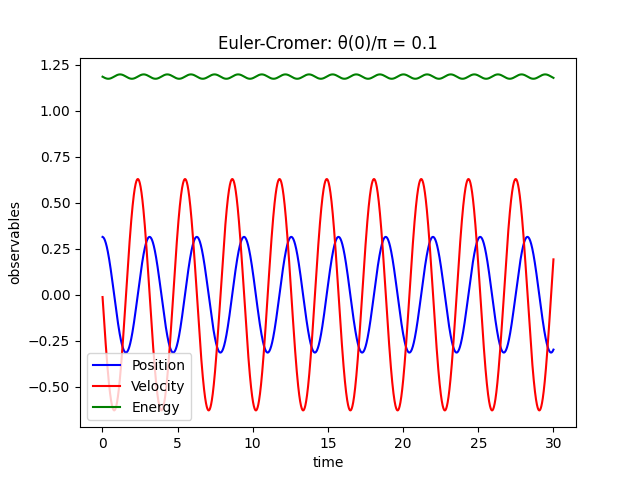
\includegraphics[width=\textwidth]{img/1-euler-cromer-0-1.png}
  \end{minipage}
  \begin{minipage}{0.45\textwidth}
    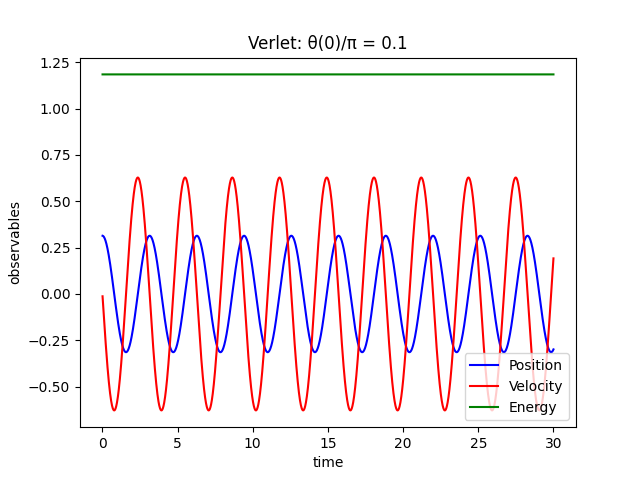
\includegraphics[width=\textwidth]{img/1-verlet-0-1.png}
  \end{minipage}
  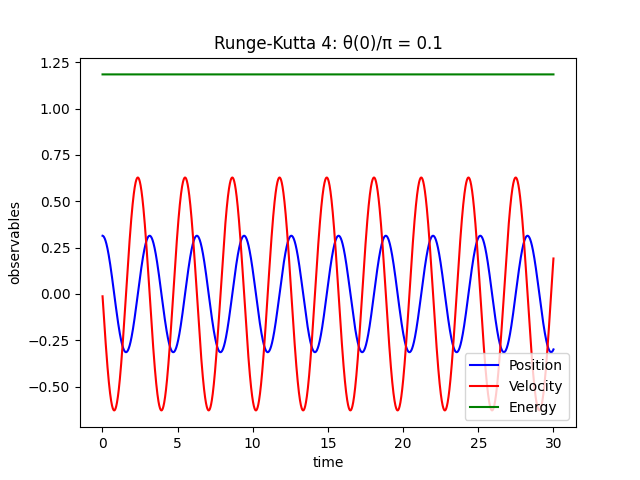
\includegraphics[scale=0.45]{img/1-runge-kutta-0-1.png}
\end{figure}

Shown above is the pendulum simulated with all three methods, with an integrator timestep of 0.01.
With Euler-Cromer, the energy of the system oscillates back and forth as it swings. This was also the case
when using the other initial condition, $\theta(0)/\pi = 0.5$.

Although Runge-Kutta has a higher order accuracy than velocity Verlet, the former usually isn't preferable
for use with physical simulations. This is due to the method not conserving energy properly, slightly
distorting it over time. This can be seem exemplified in the following figure, where Runge-Kutta and velocity
Verlet has been used to simulate the pendulum over 10 times the duration, with a timestep of $0.2$:

\begin{figure}[!ht]
  \centering
  \begin{minipage}{0.45\textwidth}
    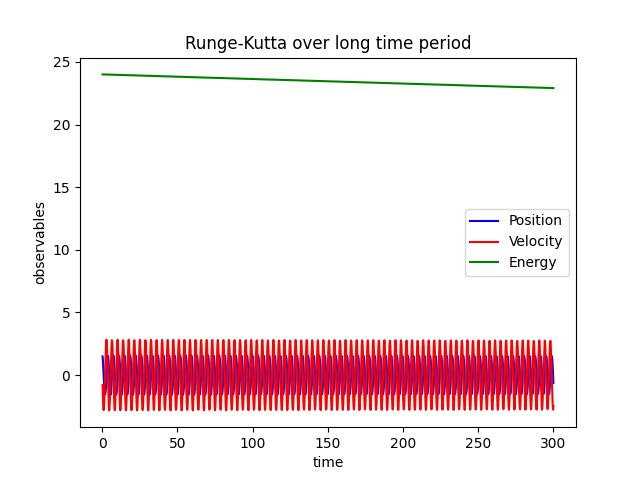
\includegraphics[width=\textwidth]{img/1-runge-kutta-long.png}
  \end{minipage}
  \begin{minipage}{0.45\textwidth}
    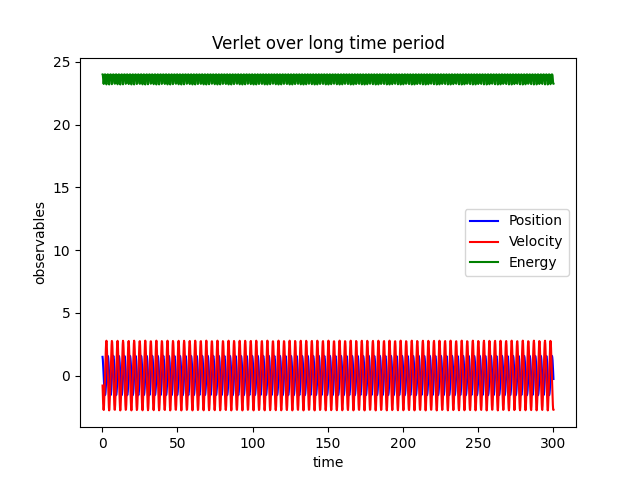
\includegraphics[width=\textwidth]{img/1-verlet-long.png}
  \end{minipage}
\end{figure}

The bigger timestep causes the simulation to be less accurate. In general we see the same behavior on the
pendulum, but the total energy slowly decreases over time when integrating with Runge-Kutta. Velocity Verlet
doens't have this issue, since it's been specificly engineered to be energy conserving, meaning it's the preferred
integrator of choice to use when running physical simulations where the timestep cannot be made arbitrarily small.


\section*{Exercise 1.2}

To determine the period time $T$ of the systems as a function of the initial position $\theta(0)$,
the simulation was run for multiple different values, ranging from $0.1$ to $3$ radians.
To calculate the period time, we look at the velocity data and note any points where it's zero. This gives 
the set of all points where the oscillator is turning around. The period time can then be calculated as the
difference of any two points separated by another one. To have a point of reference, the perturbation series
was given as the following:

\begin{equation}
  T = 2 \pi \sqrt{\frac{l}{g}} \left(1 + \frac{1}{16} \theta^2(0) + \frac{11}{3072} \theta^4(0) + \frac{173}{737280} \theta^6(0) \right)
\end{equation}

Graphing the period time for both types of systems as well as the equation above yields
\begin{figure}[!ht]
  \centering
  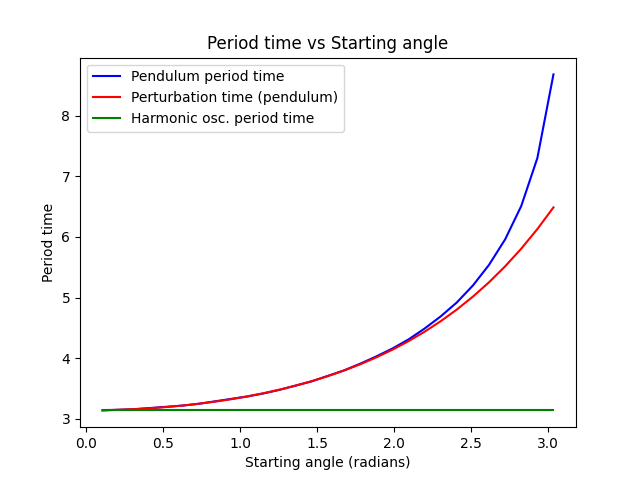
\includegraphics[scale=0.6]{img/2-period-time.png}
\end{figure}

\FloatBarrier

where we note that the period time for the harmonic oscillator is constant, regardless of the starting angle.
The period time increasing when we increase the starting angle makes sense since for the large angles, the force
applied on the pendulum won't be inline with the path of motion. The perturbation series doesn't align perfectly
with the pendulum since it is only an approximation with a finite number of terms. The more terms one would add,
the more accurate it would follow the pendulum plot.

\section*{Exercise 1.3}

Plotting $x(t)$, $v(t)$ and $E(t)$ of the damped harmonic oscillator equation with the provided values yields

\begin{figure}[!ht]
  \centering
  \begin{minipage}{0.45\textwidth}
    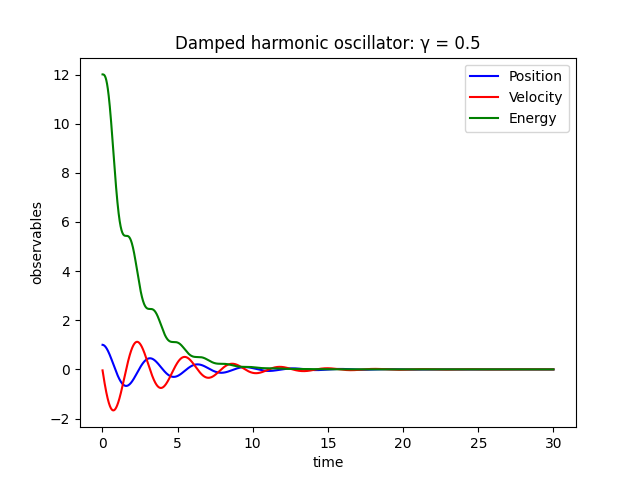
\includegraphics[width=\textwidth]{img/3-gamma-low.png}
  \end{minipage}%
  \begin{minipage}{0.45\textwidth}
    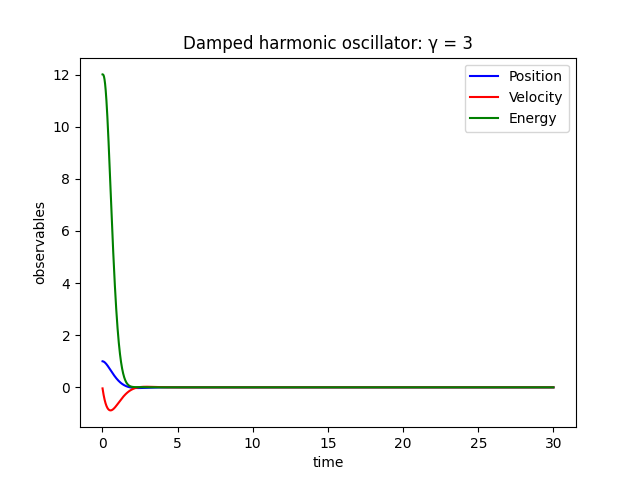
\includegraphics[width=\textwidth]{img/3-gamma-high.png}
  \end{minipage} 
\end{figure}

In the first case, the system still has time to oscillate before completely damping out. In the second case, the 
damping is so strong that the system almost instantly falls back to its stable point.

In order to estimate the relaxation time $\tau$, we need to locate the point where the envelope of the amplitude
reaches $e^{-1} \approx 37\%$ of it's original value. This was computed by looking at the amplitude of the peaks of the position,
thus not interpolating any function to give an even more detailed answer. The results are as follows:

\begin{figure}[!ht]
  \centering
  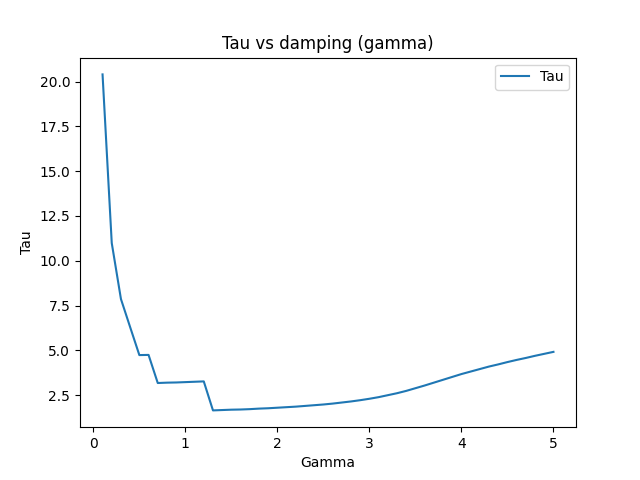
\includegraphics[scale=0.6]{img/3-tau-gamma.png}
\end{figure}

\FloatBarrier

As $\gamma$ remains small, the system is free to oscillate and takes quite some time to settle. As $\gamma$ increases,
the damping effect quickly becomes apparent, with the system settling in in about 10\% of the original time it took
to settle. Next, as gamma becomes large, the system is overdamped, meaning there are no peaks and the system actually
takes longer to settle due to movement being very constrained. The sharp steps in the graph around 0.5 to 1.3 is
caused by the method of computation. The first peak to fulfull the requirements of being $37\%$ of the original
remains the first one to fulfill the requirements for multiple values of $\gamma$. Should the peaks have been
interpolated to an exponential function, one would expect to see a smoother curve, but not see it rise slowly again
due to the significant overdampening.

In order to find the critical damping $\gamma_c$, we slowly increase $\gamma$ and check the positional data until we
find a simulation where every position in the data is positive. This process yields $\gamma_c$ to be 4.

\section*{Exercise 1.4}

Plotting the phase portrait of this system results in the following. Note that the scale on second graph's axes is
slightly different to the first one, as a consequence of how the zoom was performed.

\begin{figure}[!ht]
  \centering
  \begin{minipage}{0.45\textwidth}
    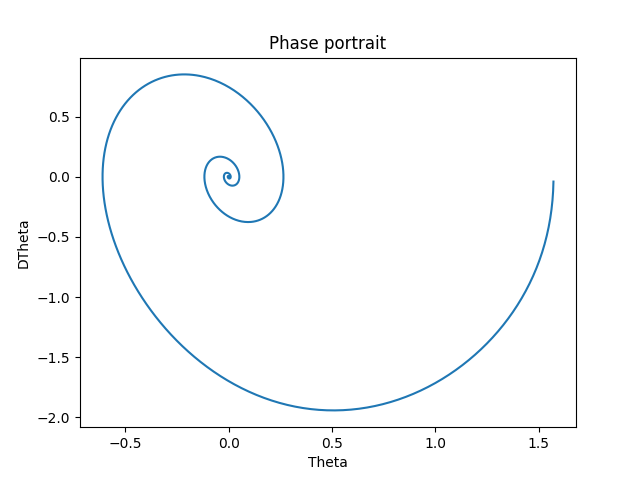
\includegraphics[width=\textwidth]{img/4-phaseportrait.png}
  \end{minipage}
  \begin{minipage}{0.45\textwidth}
    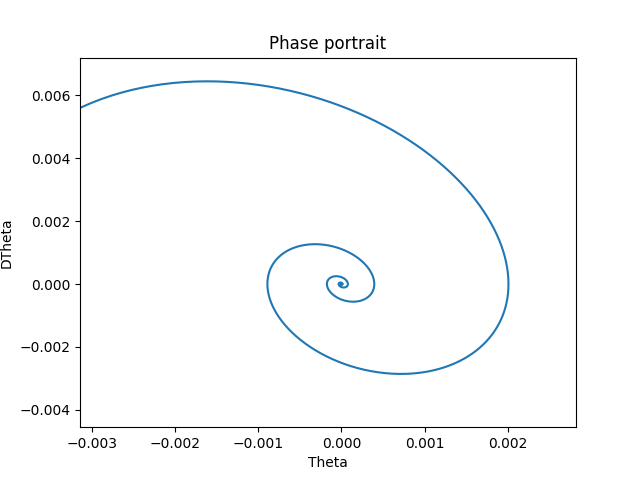
\includegraphics[width=\textwidth]{img/4-phaseportrait-zoom.png}
  \end{minipage}
\end{figure}

The phase space has some fractal-like qualities to it, ever homing in on the point $(0, 0)$. Due to the energy level of
the system being non-zero, both measures cannot equal zero simultaneously. The damping factor ensures the system is always
slowly losing energy, causing the phase to inch in on the origin in a spiral like fashion, meaning the pendulum's envelope
of movement would slowly shrink as it stabilizes towards equilibrium. Of course, in a simulation like this compared to
a physical pendulum in the real world, the physical pendulum would stop moving way earlier compared to the simulation.
Some reasons for this are that the simulation doesn't account for other external forces and factors that might be affecting
the pendulum. Forces like air resistance and friction would cause the system to have more dampening forces, meaning the
the phase portrait would converge on the origin faster.

\section*{Exercise 1.5}

\subsection*{Part a and b}

Exploring the pendulum's behavior with the energies $E = 1$, $15$, and $40$, it's clear that with $E = 1$ there's
not much going on. All the trajectories appear to be regular and the system isn't showing any signs of chaos. Jumping
up to $E = 15$, the system is starting to show some signs of chaotic behavior, albeit being stable most of the time.
The regular patterns in the energy diagram sometimes disappears, in favor of more erratic movement. At $E = 40$, chaos
ensues, literally. The phase portraits exemplifies this:

\begin{figure}[!ht]
  \centering
  \begin{minipage}{0.45\textwidth}
    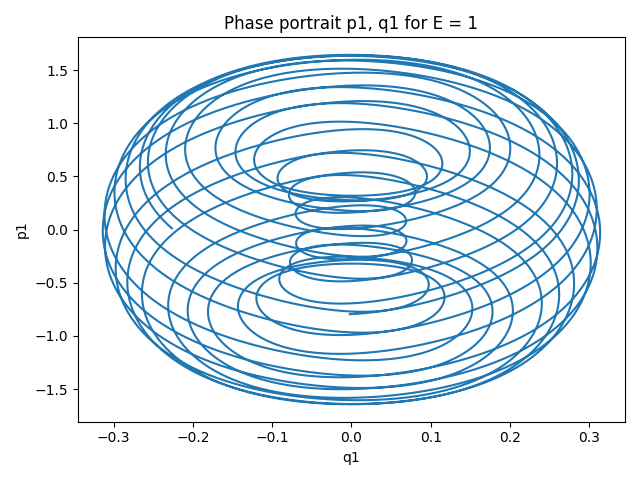
\includegraphics[width=\textwidth]{img/5-p1q1-1.png}
  \end{minipage}
  \begin{minipage}{0.45\textwidth}
    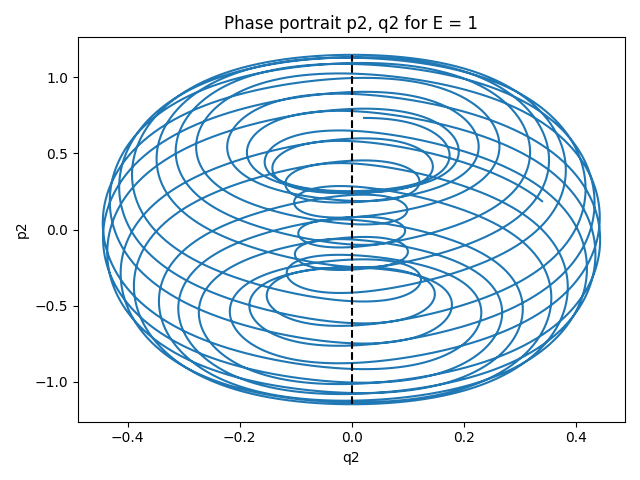
\includegraphics[width=\textwidth]{img/5-p2q2-1.png}
  \end{minipage}
\end{figure}
\begin{figure}[!ht]
  \centering
  \begin{minipage}{0.45\textwidth}
    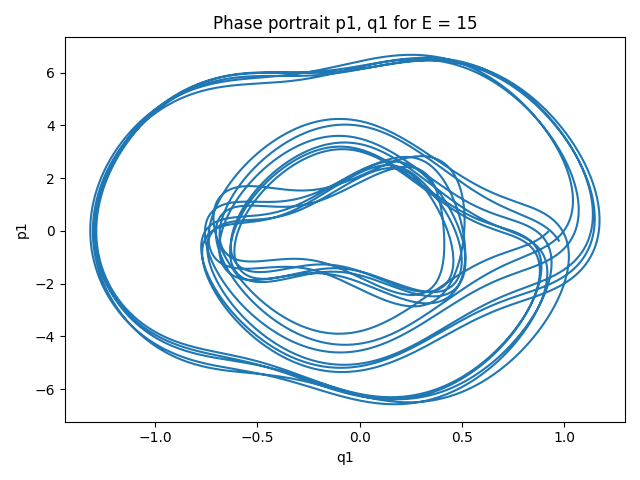
\includegraphics[width=\textwidth]{img/5-p1q1-15.png}
  \end{minipage}
  \begin{minipage}{0.45\textwidth}
    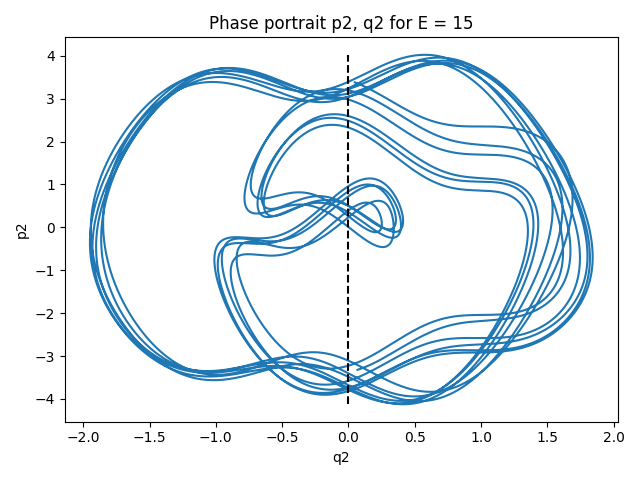
\includegraphics[width=\textwidth]{img/5-p2q2-15.png}
  \end{minipage}
\end{figure}
\begin{figure}[!ht]
  \centering
  \begin{minipage}{0.45\textwidth}
    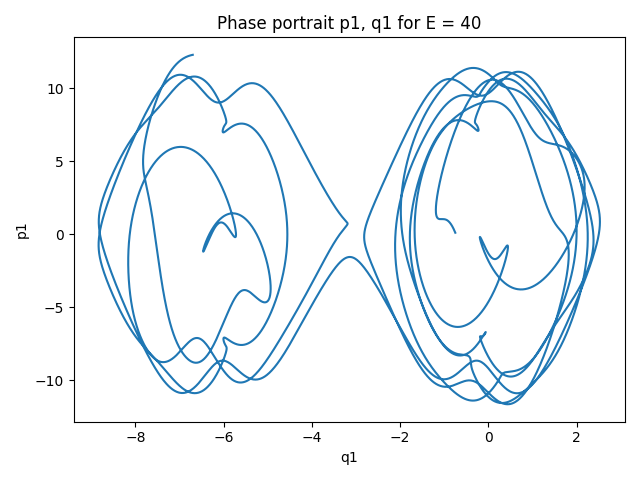
\includegraphics[width=\textwidth]{img/5-p1q1-40.png}
  \end{minipage}
  \begin{minipage}{0.45\textwidth}
    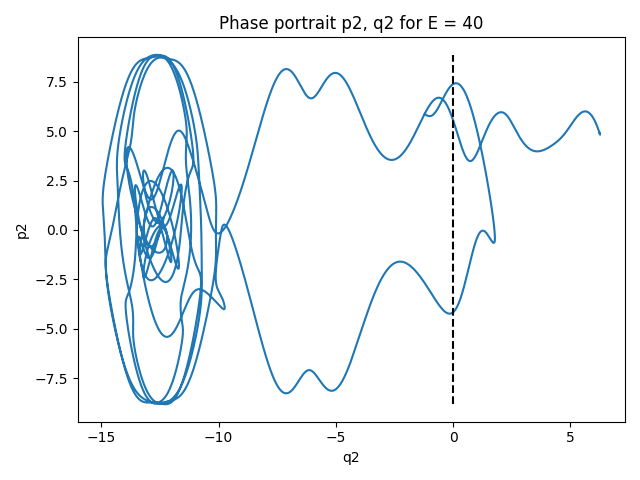
\includegraphics[width=\textwidth]{img/5-p2q2-40.png}
  \end{minipage}
\end{figure}

\FloatBarrier

At $E = 1$, there are no irregularities and all lines lie neatly in a defined pattern. As the energy increases,
some chaotic movement can be seen, though the double pendulum still mostly behaves regularly. It's very dependant
on the initial conditions, with some conditions showing signs of more chaotic patterns than others. At $E = 40$, one
cannot make out any patterns.

Drawing the phase space diagrams allows for quicker assensment if the system displays chaotic behavior than simply looking
at an animation. Regular patterns are easily made out, but chaotic behavior is (personally) made out about as easily by
looking at a phase space compared to just looking at the animation.

\subsection*{Part c}

Poincaré plots can be drawn by plotting $p_1$ vs $q_1$ when $p_2 = 0$ and $q_2 > 0$. To begin, we will replicate the plot shown
in Figure 6.13 from Lecture 1. This was done by using the initial conditions $[0, 0, 0, 0]$ and $[1.1, 0, 0, 0]$. This yields

\begin{figure}[!ht]
  \centering
  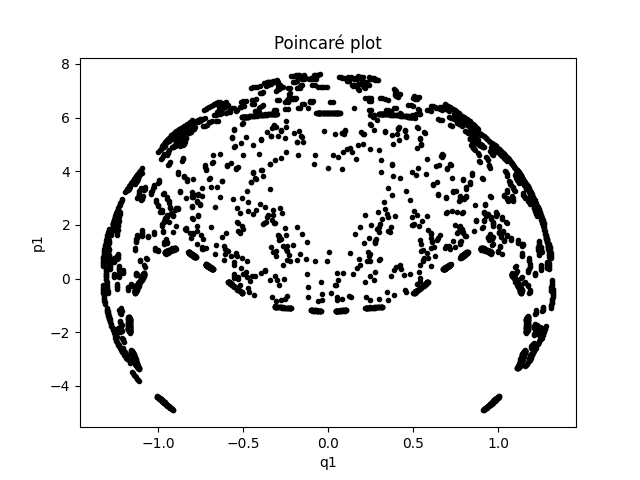
\includegraphics[scale=0.6]{img/replica.png}
\end{figure}

Overlaying five different initial conditions onto the same plot and running the simulation for the energy levels $E = 1$,
$15$ and $40$ yields the following:

\begin{figure}[!ht]
  \centering
  \begin{minipage}{0.4\textwidth}
    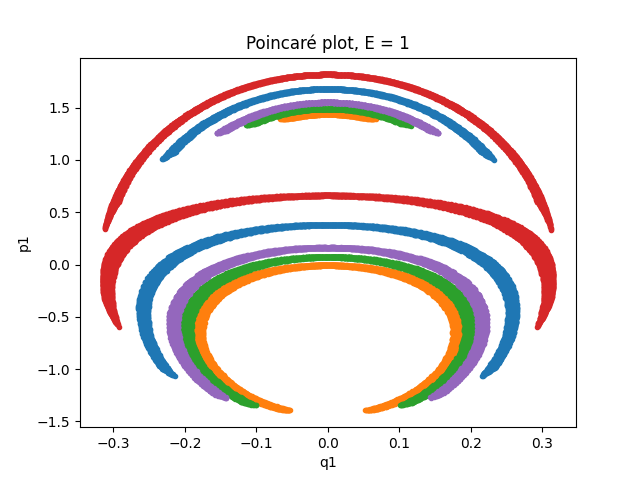
\includegraphics[width=\textwidth]{img/poincare-1.png}
  \end{minipage}
  \begin{minipage}{0.4\textwidth}
    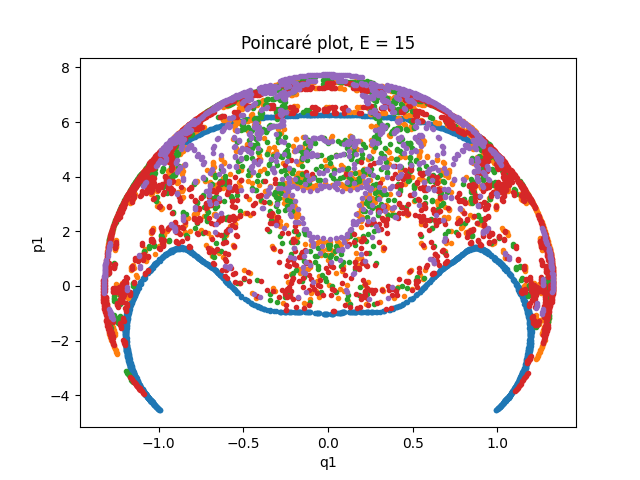
\includegraphics[width=\textwidth]{img/poincare-15.png}
  \end{minipage}
  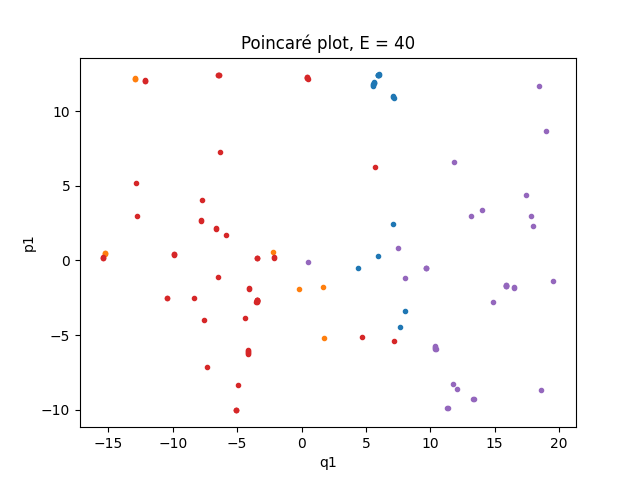
\includegraphics[scale=0.4]{img/poincare-40.png}
\end{figure}

Here it's very apparent that at low energy levels in the system, the pendulum behaves calmly and displays no tendencies
for chaotic behavior, due to the points plotted for every simulation sticking close together in well-defined strokes.
As the energy increases to $E = 15$, chaotic behavior starts to emerge, with points being plotted at seemingly random spots
within some boundary. Still though, one can clearly decuce some apparent lines in the plot, meaning the system is only
displaying partially chaotic behavior. At $E = 40$ though, the system is so chaotic that no patterns emerge on the plot.
With that being said, a prominent error factor here is the condition $p_2 = 0$. In the simulation, the variable $p_2$ never
takes on the true value $0$, meaning one has to specificly a bound for which the variable is small enough for it to count
as being zero. The pendulum now moves so fast and changes its velocity rapidly enough to not allow the simulation to detect
this particular state. If the bound was to be increased (lowering the accuracy of the plot), more dots would appear and
perhaps by then, some faint pattern may be spotted.

\subsection*{Part d}

Iterating through different energy values, the first energy level to show traces of chaotic behavior is $E = 12$, where the
first seemingly random spots appear on the plot. Shown below are the Poincaré plots for $E = 11$ and $12$, where some chaotic
trajectories first appear.

\begin{figure}[!ht]
  \centering
  \begin{minipage}{0.4\textwidth}
    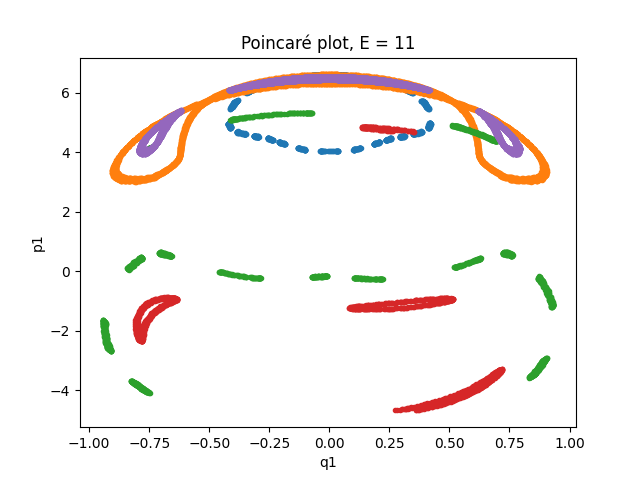
\includegraphics[width=\textwidth]{img/poincare-11.png}
  \end{minipage}
  \begin{minipage}{0.4\textwidth}
    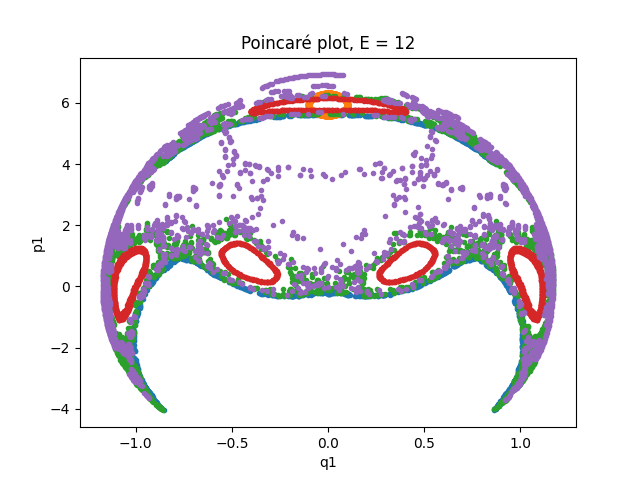
\includegraphics[width=\textwidth]{img/poincare-12.png}
  \end{minipage}
\end{figure}

\end{document}